\documentclass[problem]{mcs}

\begin{pcomments}
  \pcomment{FP_directed_graphs_and_probability} %\pcomment{from: S09.cp7r}
  \pcomment{prepared in Fall'11 for the final exam by S. Dwevidi}
\end{pcomments}

\pkeywords{
  digraphs
  DAGs
  probability
}

%%%%%%%%%%%%%%%%%%%%%%%%%%%%%%%%%%%%%%%%%%%%%%%%%%%%%%%%%%%%%%%%%%%%%
% Problem starts here
%%%%%%%%%%%%%%%%%%%%%%%%%%%%%%%%%%%%%%%%%%%%%%%%%%%%%%%%%%%%%%%%%%%%%

\begin{problem}
\bparts Let $\mathcal{G}$ be the simple graph shown in Figure ~\ref{fig:simple_graph}.

\begin{figure}[here]
\begin{center}
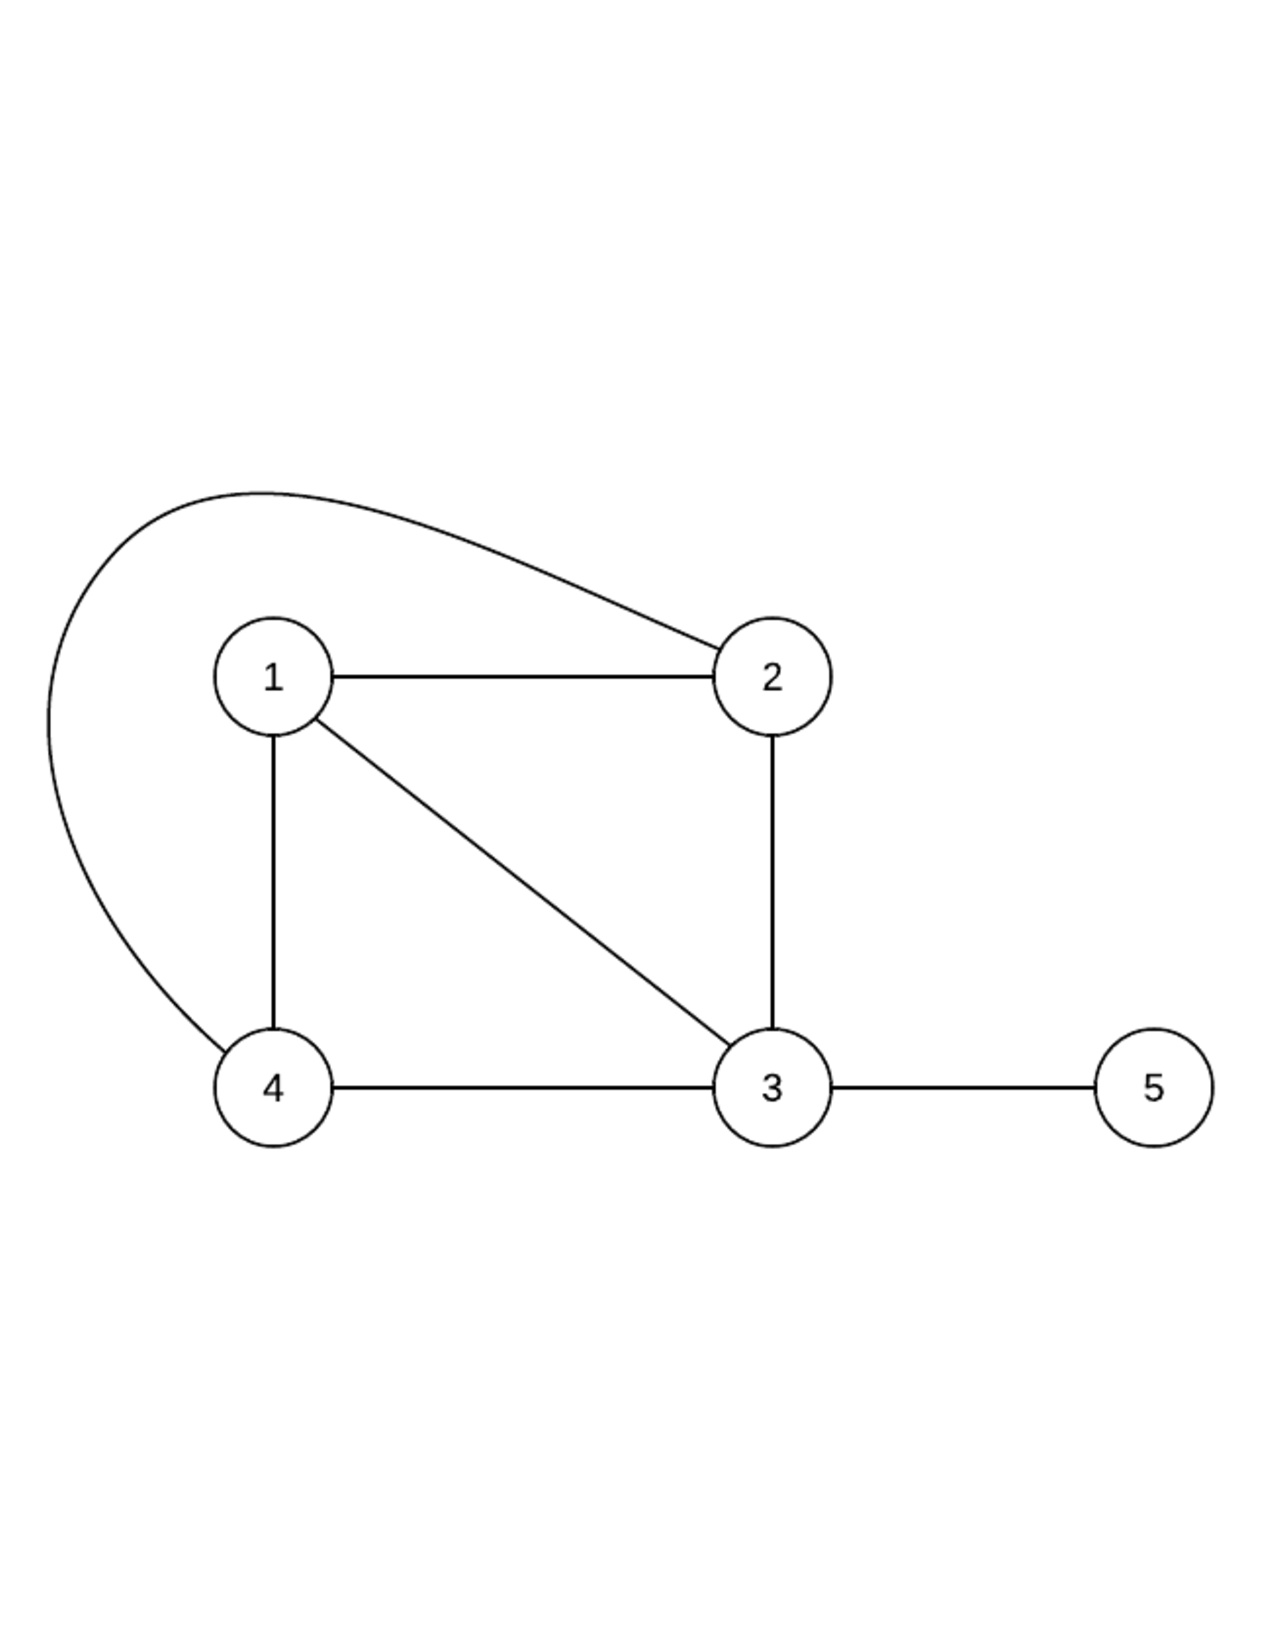
\includegraphics[scale=0.7]{simple_graph.jpg} 
%\includegraphics[width=6in,height=7in]{mq1.jpg}
\end{center}
\caption{Simple graph $\mathcal{G}$}
\label{fig:simple_graph}
\end{figure}

Construct a directed graph $\mathcal{G}_{dir}$ from the simple graph
$\mathcal{G}$ by choosing the direction of each directed edge
independentally with each direction equally likely.  Define the events:
\begin{align*}
T_1 \eqdef 123 \text{ is a directed cycle},\\
T_2 \eqdef 134 \text{ is a directed cycle},\\
T_3 \eqdef 124 \text{ is a directed cycle},\\
T_4 \eqdef 234 \text{ is a directed cycle}.
\end{align*}

\ppart What is $\pr{T_1}$? \examrule, $\pr{T_2}$? \examrule $\pr{T_3}$?
\examrule,  $\pr{T_4}?$ \examrule.

\begin{solution}
\[
\pr{T_1}= \pr{T_2}=\pr{T_3}= \pr{T_4} = \frac{2}{2^3} = \frac{1}{4}.
\]
\end{solution}

\ppart Find the probability that $\mathcal{G}_{dir}$ is a DAG
(directed acyclic graph).

\begin{solution}
Using Inclusion-Exclusion principle,
\begin{align*}
\pr{\mathcal{G}_{dir} \text{ is a DAG}}
   & = 1 - \pr{T_1 \union T_3 \union T_3 \union T_4}\\
   & = 1 - \sum_{i=1}^{4} \pr{T_i} + \sum_{i\neq j} \pr{T_i \intersect T_j} -
           \sum_{i\neq j \neq k} \pr{T_i \intersect T_j \intersect T_k} +
           \pr{T_1 \intersect T_2 \intersect T_3 \intersect T_4}\\
   & = 1 - 4 \cdot \frac{1}{4} + 6 \cdot \frac{1}{16} - 0+ 0\\
   & = \frac{3}{8}
\end{align*}

Observe that,
\begin{align*}
\pr{T_i \intersect T_j} = \frac{2}{2^5} & \text{ for $i \neq j$},\\
\pr{T_i \intersect T_j \intersect T_k} =0 & \text{for $i \neq j \neq k$, and}\\
\pr{T_1 \intersect T_2 \intersect T_3 \intersect T_4} = 0.
\end{align*}
\end{solution}

\ppart Find the minimum DAG with the same positive walk relation as
the DAG in Figure ~\ref{fig:directed_graph}.

\begin{figure}[here]
\begin{center}
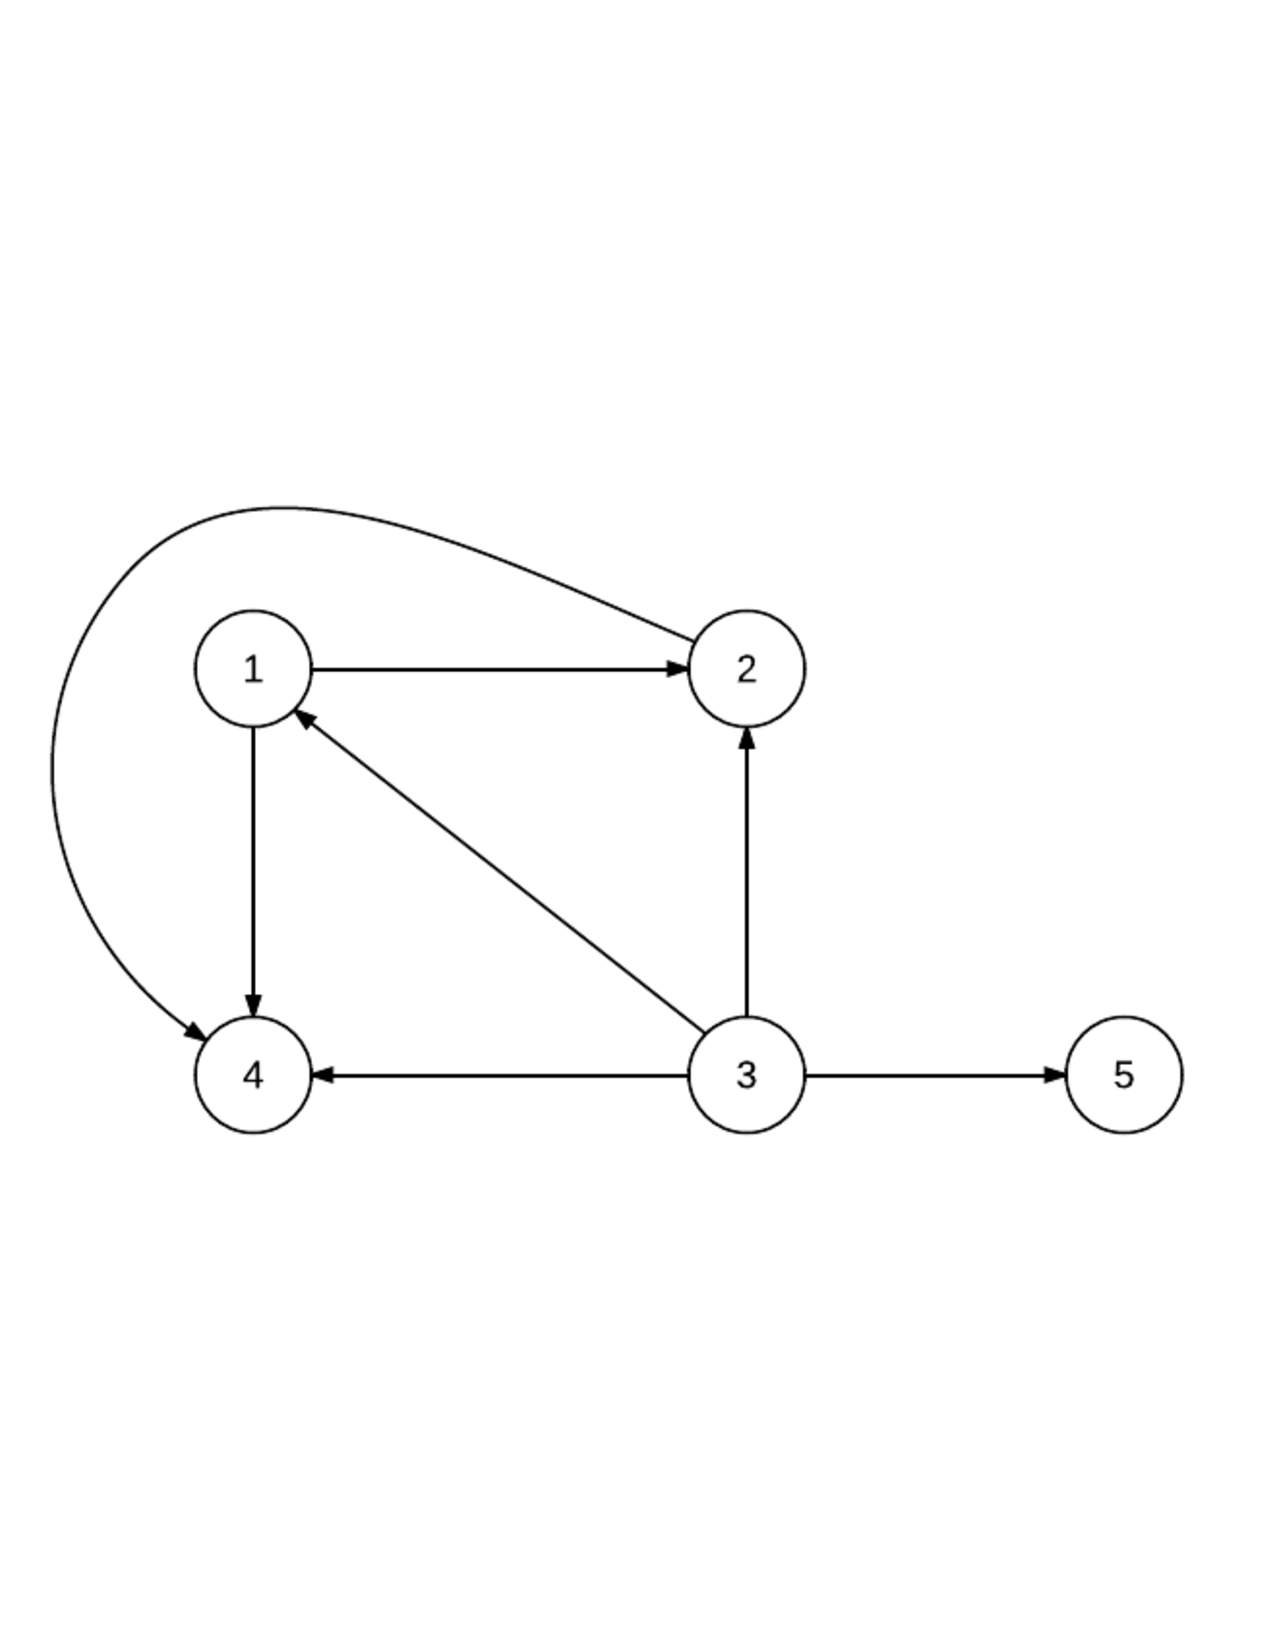
\includegraphics[scale=0.7]{dir_graph.png} 
%\includegraphics[width=6in,height=7in]{mq1.jpg}
\end{center}
\caption{DAG}
\label{fig:directed_graph}
\end{figure}

\begin{solution}
After removing edges $\diredge{3}{2}$ and $\diredge{3}{4}$, we get the minimum DAG.
\end{solution}

\ppart Find a maximal antichain for the DAG in Figure ~\ref{fig:directed_graph}.

\begin{solution}
There are multiple maximal antichains. $\set{1,5}$, $\set{2,5}$, $\set{4,5}$, etc.
\end{solution}

\eparts

\end{problem}

%%%%%%%%%%%%%%%%%%%%%%%%%%%%%%%%%%%%%%%%%%%%%%%%%%%%%%%%%%%%%%%%%%%%%
% Problem ends here
%%%%%%%%%%%%%%%%%%%%%%%%%%%%%%%%%%%%%%%%%%%%%%%%%%%%%%%%%%%%%%%%%%%%%

\endinput
